Closed loop simulations -- with the control logic of the zigzag test -- were used to predict the model test experiments. Comparisons of these predictions are shown in \autoref{fig:closed_loop_zigzag10} and \autoref{fig:closed_loop_zigzag20}. The drift angle $\beta$, heading angle $\psi$, and yaw rate $r$, are in good agreement with the experiments for all the models. The Abkowitz ID does however seems to have a faster response time.
\begin{figure}[h]
    \centering
    \includesvg[width=\columnwidth]{figures/results.closed_loop_zigzag10.svg}
    \caption{Results from a zigzag10/10 model test compared with closed loop simulations.}
    \label{fig:closed_loop_zigzag10}
\end{figure}
\begin{figure}[h]
    \centering
    \includesvg[width=\columnwidth]{figures/results.closed_loop_zigzag20.svg}
    \caption{Results from a zigzag20/20 model test compared with closed loop simulations.}
    \label{fig:closed_loop_zigzag20}
\end{figure}
Before assessing the physical correctness of the ID regression models, the physical correctness of the Reference model was first be assessed. Standard manoeuvring model tests were used for this purpose. As a first step, total forces and moments from the model test were estimates with inverse dynamics (see \autoref{sec:inverse_dynamics}). These forces were compared with corresponding forces predicted with the Reference model. 
\autoref{fig:VCT_regression_ID} shows such a comparison for a zigzag20/20 model test. The first graph shows the rudder signal $\delta$ together with drift angle $\beta$ and yaw rate $r$. A comparison of sway force $Y_D$ and yawing moment $N_D$ are shown in the other two graphs. The forces and moments predicted with the Reference model were in reasonable agreement with the forces from the experiment. There were small deviations, where the Reference model over predicted the forces and moments in the peaks -- in the ends of the counter rudder excitations. 
The predicted force signals had the same general shape as the experimental forces, which implies that the Reference model captures most of the essential physics involved in the experiment.
\autoref{fig:ID_regression_ID_N} shows the yawing moments for one of the zigzag20/20 tests predicted with the models. The yawing moment from the zigzag experiment, estimated with inverse dynamics, has also been added to these graphs -- as a second reference of the total forces. It seems that the the yawing moments are similar for all models and the experimental data. It can also be seen that the Reference model and Semi-empirical ID predicts the exact same rudder yawing moment $N_R$, since they both use the same deterministic semi-empirical rudder model -- the yawing moments from the hull $N_H$ are therefore similar for these models. The rudder yawing moment from the Abkowitz ID is however very different. The regression has thus been forced to also make the yawing moments from the hull $N_H$ to be very different -- so that the total yawing moment adds up to be correct. This means that the total yawing moment is the same for all models, but the decomposition to hull and rudder moments turns out to be very different.
\begin{figure}[h]
    \centering
    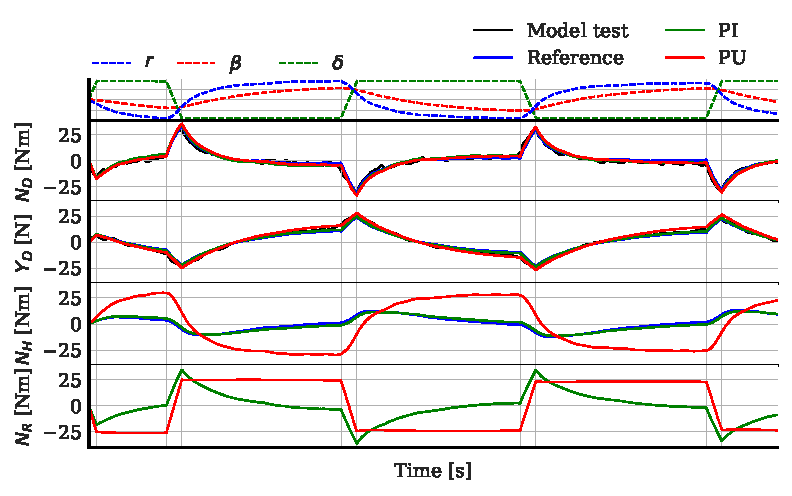
\includegraphics[width=\columnwidth]{figures/results.ID_zigzag10.pdf}
    \caption{Inverse dynamics estimations of $Y_D$, and $N_D$ during a zigzag10/10 model test compared with model predictions.}
    \label{fig:ID_regression_ID_N}
\end{figure}
\begin{figure}[h]
    \centering
    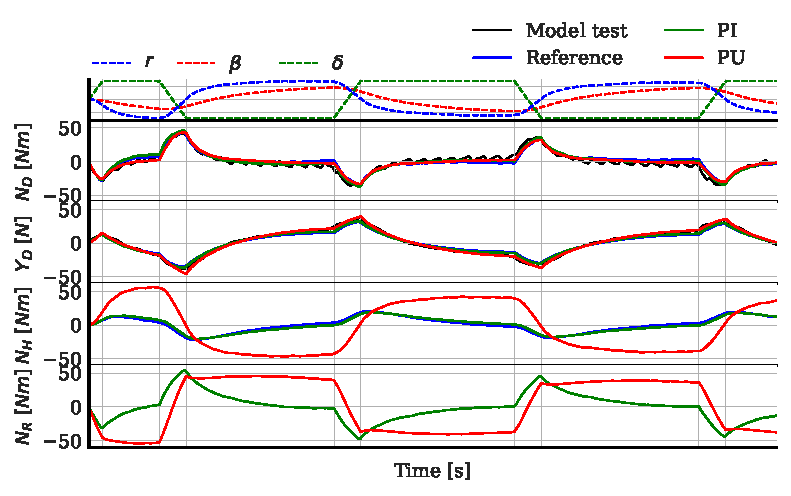
\includegraphics[width=\columnwidth]{figures/results.ID_zigzag20.pdf}
    \caption{Inverse dynamics estimations of $Y_D$, and $N_D$ during a zigzag20/20 model test compared with model predictions.}
    \label{fig:ID_regression_ID_N}
\end{figure}

The hull force model can be closer examined by decomposing the individual parameter contributions. \autoref{fig:ID_regression_N_decomposition} shows the parameter decomposition for the two models together with the Reference model. The graphs show the joined contributions for parameters related to drift ($N_v+N_{vvv}$), yaw rate ($N_r+N_{rrr}$), and combined drift and yaw rate ($N_{vrr}+N_{vvr}$). It seems that Semi-empirical ID has similar parameter decomposition to the Reference model with the exception of $N_{vrr}+N_{vvr}$ being very small; it seems that $N_r+N_{rrr}$ are a little bit larger to compensate.
The parameter decomposition of the Abkowitz ID is completely different, where almost the entire contribution to the hull yawing moment $N_H$ can be denoted to the yaw rate parameters $N_r+N_{rrr}$. 
\begin{figure}[h]
    \begin{center}
        \includesvg[width=\columnwidth]{figures/results.hull_force_decomposition_zigzag20.svg}
        \caption{Decomposition of hull forces and moments during a zigzag20/20 test for parameters related to drift, yaw rate the prediction models.}
        \label{fig:ID_regression_N_decomposition}
    \end{center}
\end{figure}

Possible implications of that the Abkowitz model have this physically incorrect decomposition of the hull's drift angle and yaw rate dependence will be further investigated in the next section.